% ============================================================================
% SYSTEM PIPELINE FLOWCHART - USAGE GUIDE
% ============================================================================
% This file contains instructions for using the flowchart in your paper
% ============================================================================

% ============================================================================
% PREAMBLE REQUIREMENTS
% ============================================================================
% Add these packages to your LaTeX document preamble:

\documentclass{article} % or your conference/journal class

% Required packages
\usepackage{tikz}
\usetikzlibrary{shapes.geometric, arrows.meta, positioning, fit, backgrounds}
\usepackage{graphicx}
\usepackage{amsmath}

% Optional: For better positioning in two-column layouts
\usepackage{dblfloatfix}

% ============================================================================
% USAGE INSTRUCTIONS
% ============================================================================

% Option 1: Include the full two-column flowchart
% Best for: Two-column papers (IEEE, ACM) with sufficient space
% Location: Top of page with [t] placement
% File: system_pipeline_flowchart.tex

% In your paper, use:
% % System Pipeline Flowchart for Research Paper
% Requires: \usepackage{tikz}
%          \usetikzlibrary{shapes.geometric, arrows.meta, positioning, fit, backgrounds}

\begin{figure*}[t]
\centering
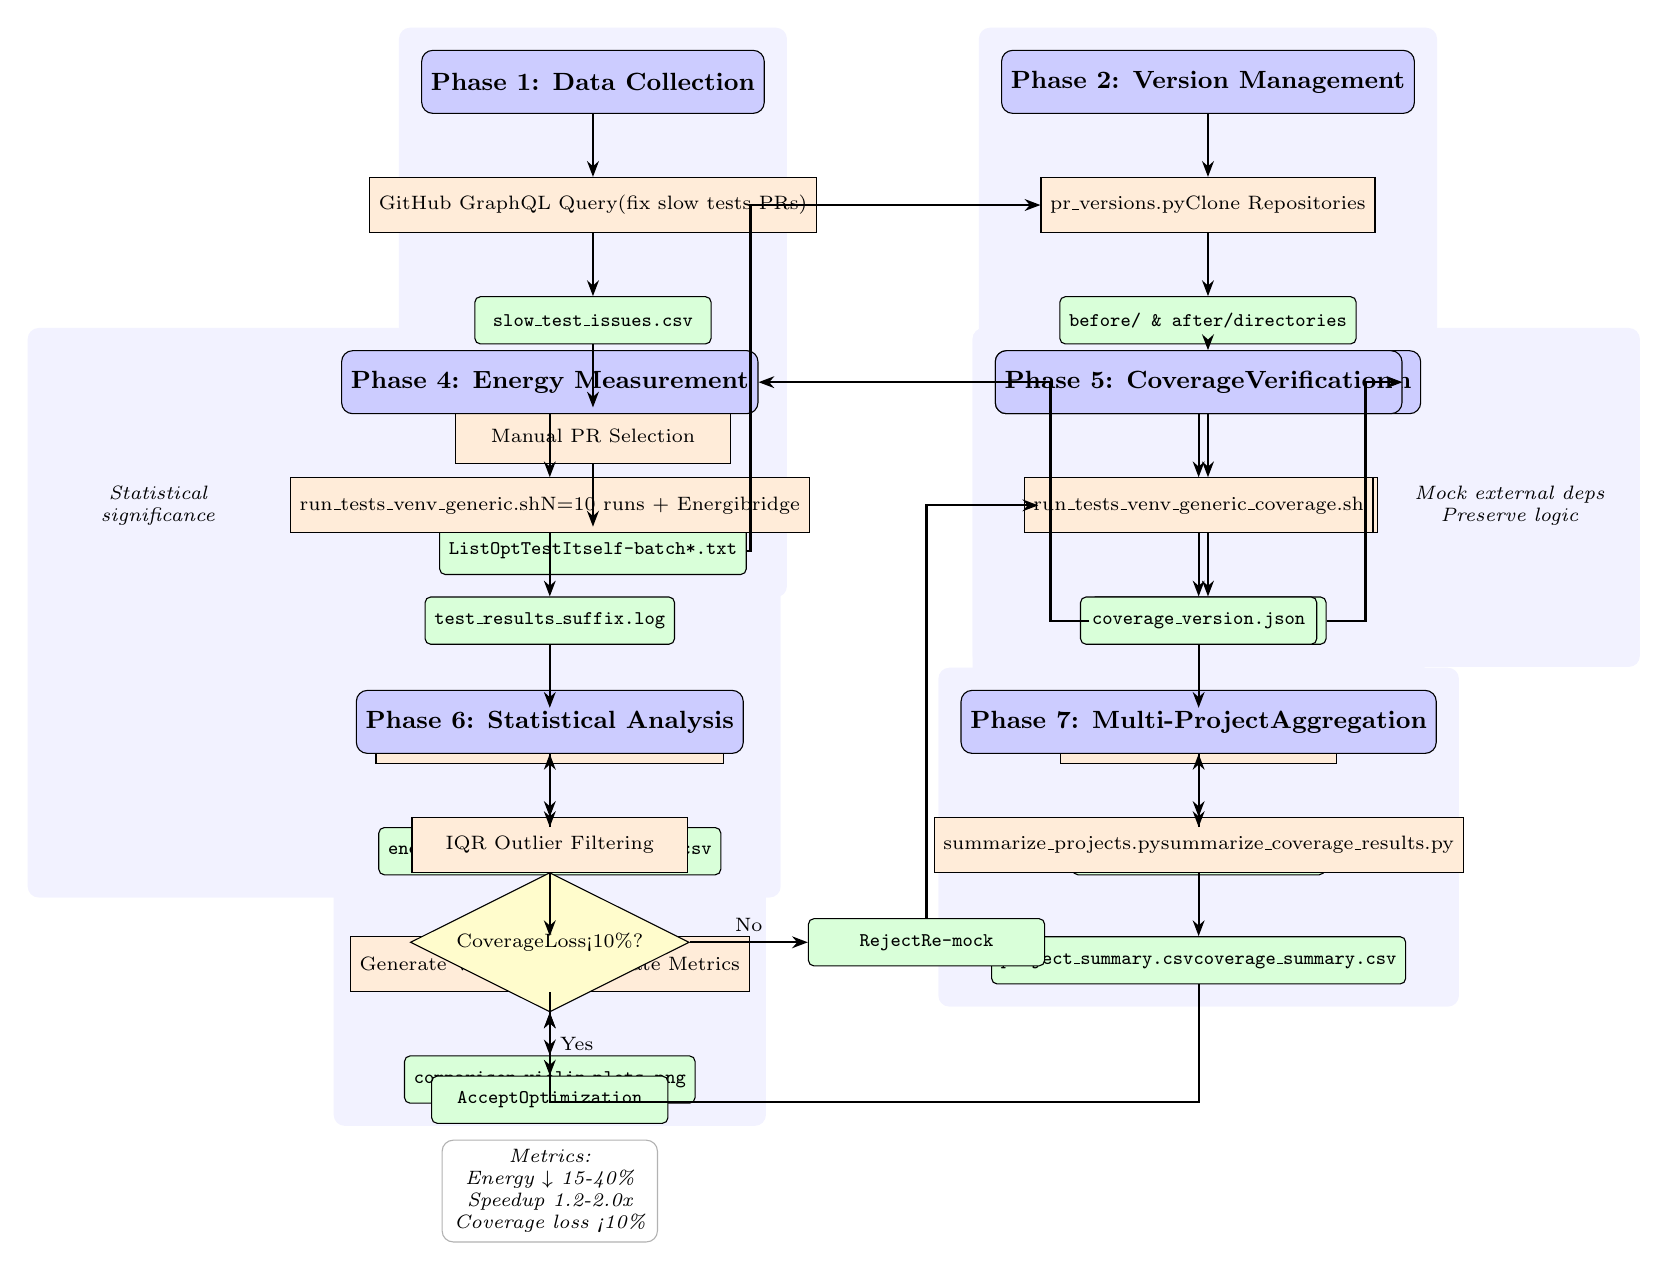
\begin{tikzpicture}[
    node distance=0.8cm and 1.2cm,
    % Style definitions
    phase/.style={rectangle, rounded corners, minimum width=3cm, minimum height=0.8cm,
                  text centered, draw=black, fill=blue!20, font=\small\bfseries},
    process/.style={rectangle, minimum width=3.5cm, minimum height=0.7cm,
                    text centered, draw=black, fill=orange!15, font=\scriptsize},
    data/.style={rectangle, rounded corners=2pt, minimum width=3cm, minimum height=0.6cm,
                 text centered, draw=black, fill=green!15, font=\scriptsize\ttfamily},
    decision/.style={diamond, aspect=2, minimum width=2.5cm, minimum height=0.8cm,
                     text centered, draw=black, fill=yellow!20, font=\scriptsize},
    arrow/.style={-{Stealth[length=2mm]}, thick},
    annotation/.style={font=\scriptsize\itshape, text width=2.5cm, align=center},
]

% Phase 1: Data Collection
\node[phase] (phase1) {Phase 1: Data Collection};
\node[process, below=of phase1] (fetch) {GitHub GraphQL Query\\(fix slow tests PRs)};
\node[data, below=of fetch] (csv) {slow\_test\_issues.csv};
\node[process, below=of csv] (select) {Manual PR Selection};
\node[data, below=of select] (batch) {ListOptTestItself-\\batch*.txt};

% Phase 2: Version Management
\node[phase, right=3cm of phase1] (phase2) {Phase 2: Version Management};
\node[process, below=of phase2] (download) {pr\_versions.py\\Clone Repositories};
\node[data, below=of download] (versions) {before/ \& after/\\directories};

% Phase 3: Mock Implementation
\node[phase, below=3cm of phase2] (phase3) {Phase 3: Mock Implementation};
\node[process, below=of phase3] (claude) {Claude Code\\+ Prompt Template};
\node[data, below=of claude] (mock) {after\_careful\_mock/};
\node[annotation, right=0.3cm of claude] (guideline) {Mock external deps\\Preserve logic};

% Phase 4: Energy Measurement
\node[phase, left=3cm of phase3] (phase4) {Phase 4: Energy Measurement};
\node[process, below=of phase4] (energi) {run\_tests\_venv\_generic.sh\\N=10 runs + Energibridge};
\node[data, below=of energi] (logs) {test\_results\_\\{suffix}.log};
\node[process, below=of logs] (parse) {parse\_results\_\\generic\_optimized.py};
\node[data, below=of parse] (energy_csv) {energy\_data.csv\\duration\_data.csv};
\node[annotation, left=0.3cm of energi] (n_runs) {Statistical\\significance};

% Phase 5: Coverage Verification
\node[phase, right=3cm of phase4] (phase5) {Phase 5: Coverage\\Verification};
\node[process, below=of phase5] (cov_run) {run\_tests\_venv\_\\generic\_coverage.sh};
\node[data, below=of cov_run] (cov_json) {coverage\_\\{version}.json};
\node[process, below=of cov_json] (compare) {compare\_coverage.py};
\node[data, below=of compare] (cov_txt) {coverage\_\\comparison.txt};

% Phase 6: Statistical Analysis
\node[phase, below=3.5cm of phase4] (phase6) {Phase 6: Statistical Analysis};
\node[process, below=of phase6] (filter) {IQR Outlier Filtering};
\node[process, below=of filter] (visualize) {Generate Violin Plots\\Calculate Metrics};
\node[data, below=of visualize] (plots) {comparison\_\\violin\_plots.png};

% Phase 7: Multi-Project Aggregation
\node[phase, below=3.5cm of phase5] (phase7) {Phase 7: Multi-Project\\Aggregation};
\node[process, below=of phase7] (summarize) {summarize\_projects.py\\summarize\_coverage\_\\results.py};
\node[data, below=of summarize] (summary) {project\_summary.csv\\coverage\_summary.csv};

% Decision Diamond
\node[decision, below=1.5cm of phase6] (decision) {Coverage\\Loss\\<10\%?};
\node[data, below=0.8cm of decision] (accept) {\textbf{Accept}\\Optimization};
\node[data, right=1.5cm of decision] (reject) {\textbf{Reject}\\Re-mock};

% Arrows - Phase 1
\draw[arrow] (phase1) -- (fetch);
\draw[arrow] (fetch) -- (csv);
\draw[arrow] (csv) -- (select);
\draw[arrow] (select) -- (batch);

% Arrows - Phase 2
\draw[arrow] (batch) -- ++(2,0) |- (download);
\draw[arrow] (phase2) -- (download);
\draw[arrow] (download) -- (versions);

% Arrows - Phase 3
\draw[arrow] (versions) -- (phase3);
\draw[arrow] (phase3) -- (claude);
\draw[arrow] (claude) -- (mock);

% Arrows - Phase 4
\draw[arrow] (mock) -- ++(-2,0) |- (phase4);
\draw[arrow] (phase4) -- (energi);
\draw[arrow] (energi) -- (logs);
\draw[arrow] (logs) -- (parse);
\draw[arrow] (parse) -- (energy_csv);

% Arrows - Phase 5
\draw[arrow] (mock) -- ++(2,0) |- (phase5);
\draw[arrow] (phase5) -- (cov_run);
\draw[arrow] (cov_run) -- (cov_json);
\draw[arrow] (cov_json) -- (compare);
\draw[arrow] (compare) -- (cov_txt);

% Arrows - Phase 6 & 7
\draw[arrow] (energy_csv) -- (phase6);
\draw[arrow] (phase6) -- (filter);
\draw[arrow] (filter) -- (visualize);
\draw[arrow] (visualize) -- (plots);
\draw[arrow] (cov_txt) -- (phase7);
\draw[arrow] (phase7) -- (summarize);
\draw[arrow] (summarize) -- (summary);

% Arrows - Decision
\draw[arrow] (plots) -- (decision);
\draw[arrow] (summary) -- ++(0,-1.8) -| (decision);
\draw[arrow] (decision) -- node[right, font=\scriptsize] {Yes} (accept);
\draw[arrow] (decision) -- node[above, font=\scriptsize] {No} (reject);
\draw[arrow] (reject) |- (claude);

% Background boxes for phases
\begin{scope}[on background layer]
    \node[fit=(phase1)(batch), fill=blue!5, rounded corners, inner sep=8pt] {};
    \node[fit=(phase2)(versions), fill=blue!5, rounded corners, inner sep=8pt] {};
    \node[fit=(phase3)(mock)(guideline), fill=blue!5, rounded corners, inner sep=8pt] {};
    \node[fit=(phase4)(energy_csv)(n_runs), fill=blue!5, rounded corners, inner sep=8pt] {};
    \node[fit=(phase5)(cov_txt), fill=blue!5, rounded corners, inner sep=8pt] {};
    \node[fit=(phase6)(plots), fill=blue!5, rounded corners, inner sep=8pt] {};
    \node[fit=(phase7)(summary), fill=blue!5, rounded corners, inner sep=8pt] {};
\end{scope}

% Metrics annotations
\node[annotation, below=0.2cm of accept, fill=white, draw=black!30, rounded corners] (metrics) {
    Metrics:\\
    Energy $\downarrow$ 15-40\%\\
    Speedup 1.2-2.0x\\
    Coverage loss <10\%
};

\end{tikzpicture}
\caption{System pipeline for evaluating energy-aware slow test optimization. The pipeline consists of seven phases: (1) identifying GitHub projects with slow test fixes, (2) downloading before/after PR versions, (3) applying mocking strategies using Claude Code, (4) measuring energy consumption across N=10 runs with Energibridge, (5) verifying test coverage preservation, (6) statistical analysis with outlier filtering, and (7) multi-project aggregation. Optimizations are accepted only if coverage loss is below 10\%.}
\label{fig:system_pipeline}
\end{figure*}


% ============================================================================

% Option 2: Include the compact single-column flowchart
% Best for: Single-column papers or space-constrained layouts
% Location: Can be placed in either column with [t] or [h] placement
% File: system_pipeline_flowchart_compact.tex

% In your paper, use:
% % Compact System Pipeline Flowchart for Research Paper (Single Column)
% Requires: \usepackage{tikz}
%          \usetikzlibrary{shapes.geometric, arrows.meta, positioning}

\begin{figure}[t]
\centering
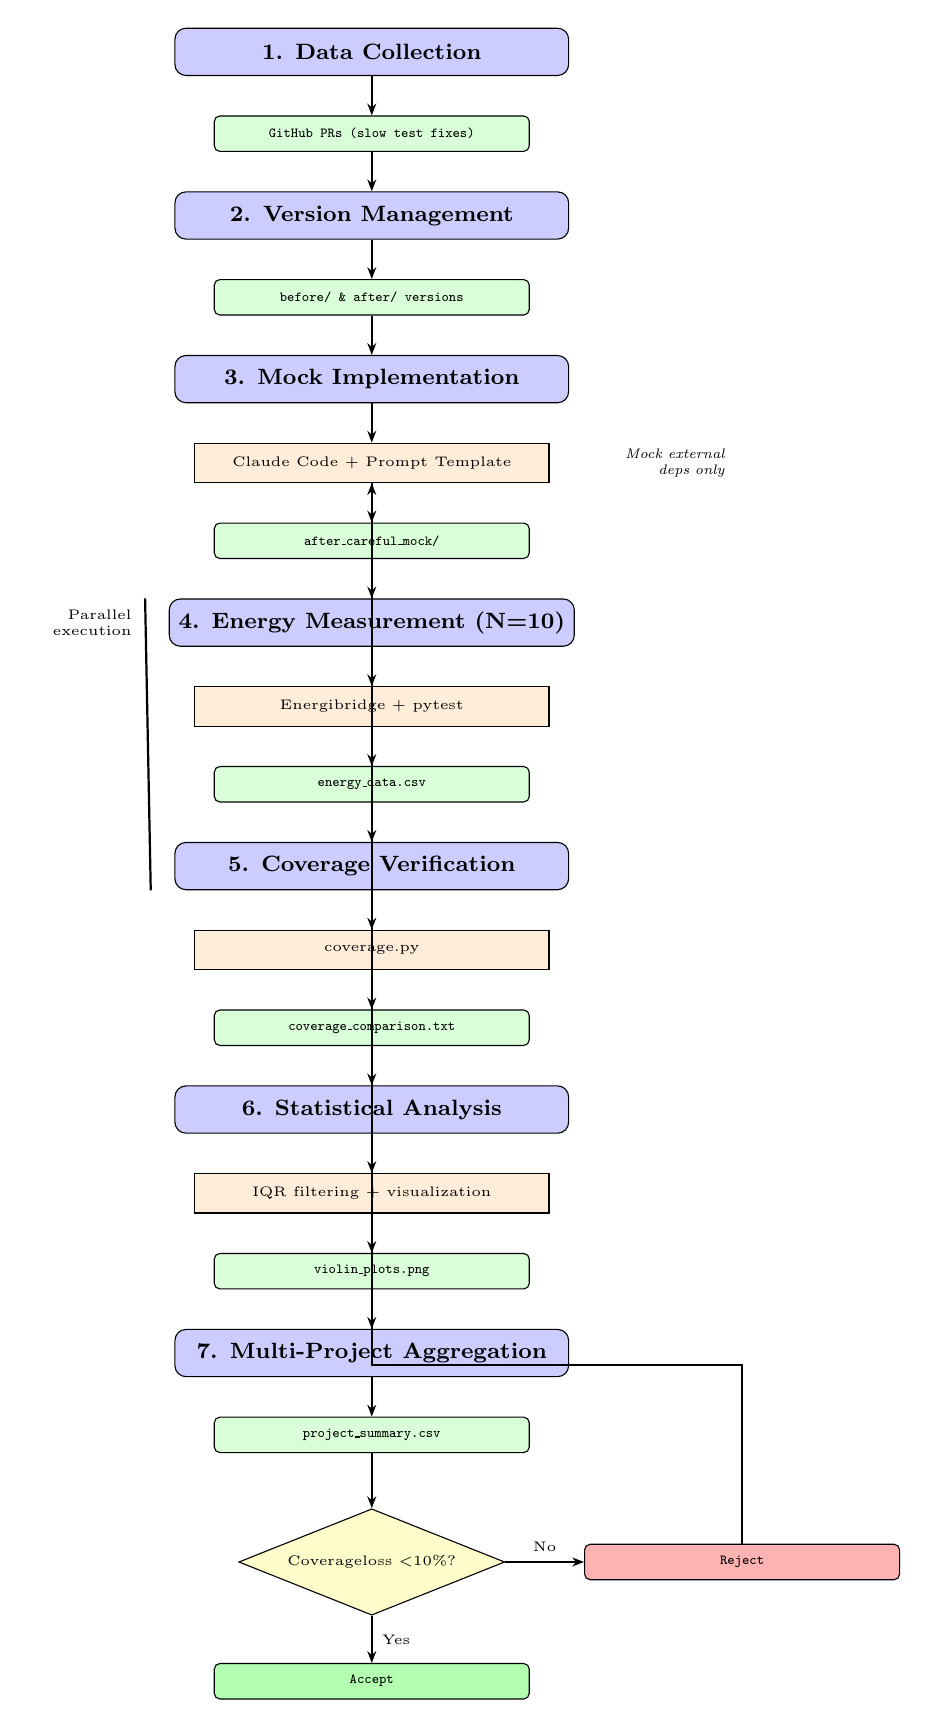
\begin{tikzpicture}[
    node distance=0.5cm,
    % Style definitions
    phase/.style={rectangle, rounded corners, minimum width=5cm, minimum height=0.6cm,
                  text centered, draw=black, fill=blue!20, font=\footnotesize\bfseries},
    process/.style={rectangle, minimum width=4.5cm, minimum height=0.5cm,
                    text centered, draw=black, fill=orange!15, font=\tiny},
    data/.style={rectangle, rounded corners=2pt, minimum width=4cm, minimum height=0.45cm,
                 text centered, draw=black, fill=green!15, font=\tiny\ttfamily},
    decision/.style={diamond, aspect=2.5, minimum width=3cm, minimum height=0.6cm,
                     text centered, draw=black, fill=yellow!20, font=\tiny},
    arrow/.style={-{Stealth[length=1.5mm]}, thick},
    annotation/.style={font=\tiny\itshape, text width=2cm, align=right},
]

% Vertical pipeline
\node[phase] (p1) {1. Data Collection};
\node[data, below=of p1] (d1) {GitHub PRs (slow test fixes)};

\node[phase, below=of d1] (p2) {2. Version Management};
\node[data, below=of p2] (d2) {before/ \& after/ versions};

\node[phase, below=of d2] (p3) {3. Mock Implementation};
\node[process, below=of p3] (pr3) {Claude Code + Prompt Template};
\node[data, below=of pr3] (d3) {after\_careful\_mock/};
\node[annotation, right=0.1cm of pr3] (a3) {Mock external\\deps only};

\node[phase, below=of d3] (p4) {4. Energy Measurement (N=10)};
\node[process, below=of p4] (pr4) {Energibridge + pytest};
\node[data, below=of pr4] (d4) {energy\_data.csv};

\node[phase, below=of d4] (p5) {5. Coverage Verification};
\node[process, below=of p5] (pr5) {coverage.py};
\node[data, below=of pr5] (d5) {coverage\_comparison.txt};

\node[phase, below=of d5] (p6) {6. Statistical Analysis};
\node[process, below=of p6] (pr6) {IQR filtering + visualization};
\node[data, below=of pr6] (d6) {violin\_plots.png};

\node[phase, below=of d6] (p7) {7. Multi-Project Aggregation};
\node[data, below=of p7] (d7) {project\_summary.csv};

\node[decision, below=0.7cm of d7] (dec) {Coverage\\loss <10\%?};
\node[data, below=0.6cm of dec, fill=green!30] (accept) {Accept};
\node[data, right=1cm of dec, fill=red!30] (reject) {Reject};

% Arrows
\draw[arrow] (p1) -- (d1);
\draw[arrow] (d1) -- (p2);
\draw[arrow] (p2) -- (d2);
\draw[arrow] (d2) -- (p3);
\draw[arrow] (p3) -- (pr3);
\draw[arrow] (pr3) -- (d3);
\draw[arrow] (d3) -- (p4);
\draw[arrow] (p4) -- (pr4);
\draw[arrow] (pr4) -- (d4);
\draw[arrow] (d4) -- (p5);
\draw[arrow] (p5) -- (pr5);
\draw[arrow] (pr5) -- (d5);
\draw[arrow] (d5) -- (p6);
\draw[arrow] (p6) -- (pr6);
\draw[arrow] (pr6) -- (d6);
\draw[arrow] (d6) -- (p7);
\draw[arrow] (p7) -- (d7);
\draw[arrow] (d7) -- (dec);
\draw[arrow] (dec) -- node[right, font=\tiny] {Yes} (accept);
\draw[arrow] (dec) -- node[above, font=\tiny] {No} (reject);
\draw[arrow] (reject) |- ++(0,2.5) -| (pr3);

% Parallel processes annotation with simple line
\draw[thick] ([xshift=-0.3cm]p4.north west) -- ([xshift=-0.3cm]p5.south west);
\node[font=\tiny, text width=1.2cm, align=right, left=0.35cm of p4] {Parallel execution};

\end{tikzpicture}
\caption{Energy-aware slow test optimization pipeline. The system evaluates test optimizations through seven automated phases, accepting optimizations only when coverage loss remains below 10\% while achieving significant energy reduction (15-40\%) and speedup (1.2-2.0$\times$).}
\label{fig:pipeline_compact}
\end{figure}


% ============================================================================
% EXAMPLE PAPER STRUCTURE
% ============================================================================

\begin{document}

\title{Energy-Aware Slow Test Optimization Using Automated Mocking}
\author{Your Name}
\maketitle

\begin{abstract}
This paper presents an automated pipeline for evaluating and optimizing slow tests in software projects...
\end{abstract}

\section{Introduction}
Software testing is crucial for quality assurance, but slow tests can significantly impact developer productivity and energy consumption...

\section{Methodology}

Our approach consists of seven phases as illustrated in Figure~\ref{fig:system_pipeline}.

% TWO-COLUMN VERSION (for IEEE, ACM double-column formats)
% System Pipeline Flowchart for Research Paper
% Requires: \usepackage{tikz}
%          \usetikzlibrary{shapes.geometric, arrows.meta, positioning, fit, backgrounds}

\begin{figure*}[t]
\centering
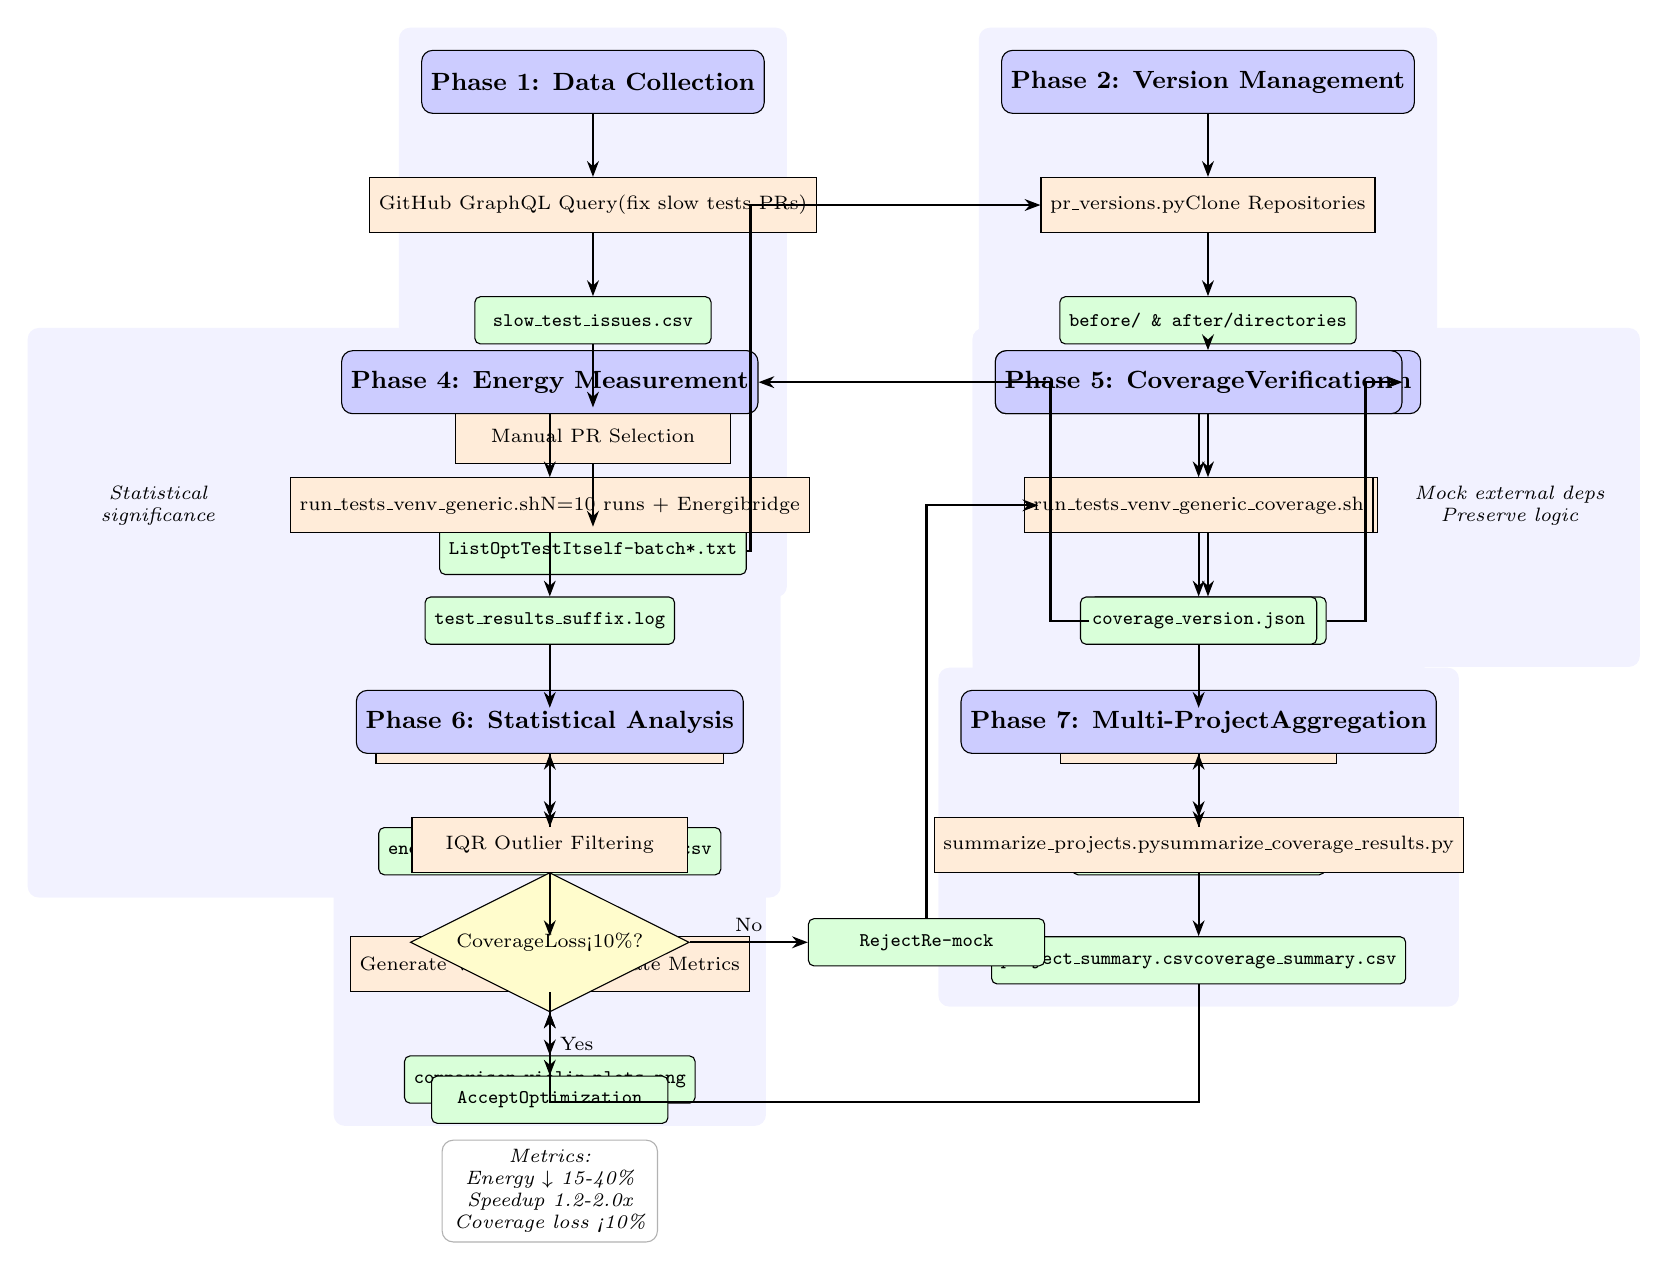
\begin{tikzpicture}[
    node distance=0.8cm and 1.2cm,
    % Style definitions
    phase/.style={rectangle, rounded corners, minimum width=3cm, minimum height=0.8cm,
                  text centered, draw=black, fill=blue!20, font=\small\bfseries},
    process/.style={rectangle, minimum width=3.5cm, minimum height=0.7cm,
                    text centered, draw=black, fill=orange!15, font=\scriptsize},
    data/.style={rectangle, rounded corners=2pt, minimum width=3cm, minimum height=0.6cm,
                 text centered, draw=black, fill=green!15, font=\scriptsize\ttfamily},
    decision/.style={diamond, aspect=2, minimum width=2.5cm, minimum height=0.8cm,
                     text centered, draw=black, fill=yellow!20, font=\scriptsize},
    arrow/.style={-{Stealth[length=2mm]}, thick},
    annotation/.style={font=\scriptsize\itshape, text width=2.5cm, align=center},
]

% Phase 1: Data Collection
\node[phase] (phase1) {Phase 1: Data Collection};
\node[process, below=of phase1] (fetch) {GitHub GraphQL Query\\(fix slow tests PRs)};
\node[data, below=of fetch] (csv) {slow\_test\_issues.csv};
\node[process, below=of csv] (select) {Manual PR Selection};
\node[data, below=of select] (batch) {ListOptTestItself-\\batch*.txt};

% Phase 2: Version Management
\node[phase, right=3cm of phase1] (phase2) {Phase 2: Version Management};
\node[process, below=of phase2] (download) {pr\_versions.py\\Clone Repositories};
\node[data, below=of download] (versions) {before/ \& after/\\directories};

% Phase 3: Mock Implementation
\node[phase, below=3cm of phase2] (phase3) {Phase 3: Mock Implementation};
\node[process, below=of phase3] (claude) {Claude Code\\+ Prompt Template};
\node[data, below=of claude] (mock) {after\_careful\_mock/};
\node[annotation, right=0.3cm of claude] (guideline) {Mock external deps\\Preserve logic};

% Phase 4: Energy Measurement
\node[phase, left=3cm of phase3] (phase4) {Phase 4: Energy Measurement};
\node[process, below=of phase4] (energi) {run\_tests\_venv\_generic.sh\\N=10 runs + Energibridge};
\node[data, below=of energi] (logs) {test\_results\_\\{suffix}.log};
\node[process, below=of logs] (parse) {parse\_results\_\\generic\_optimized.py};
\node[data, below=of parse] (energy_csv) {energy\_data.csv\\duration\_data.csv};
\node[annotation, left=0.3cm of energi] (n_runs) {Statistical\\significance};

% Phase 5: Coverage Verification
\node[phase, right=3cm of phase4] (phase5) {Phase 5: Coverage\\Verification};
\node[process, below=of phase5] (cov_run) {run\_tests\_venv\_\\generic\_coverage.sh};
\node[data, below=of cov_run] (cov_json) {coverage\_\\{version}.json};
\node[process, below=of cov_json] (compare) {compare\_coverage.py};
\node[data, below=of compare] (cov_txt) {coverage\_\\comparison.txt};

% Phase 6: Statistical Analysis
\node[phase, below=3.5cm of phase4] (phase6) {Phase 6: Statistical Analysis};
\node[process, below=of phase6] (filter) {IQR Outlier Filtering};
\node[process, below=of filter] (visualize) {Generate Violin Plots\\Calculate Metrics};
\node[data, below=of visualize] (plots) {comparison\_\\violin\_plots.png};

% Phase 7: Multi-Project Aggregation
\node[phase, below=3.5cm of phase5] (phase7) {Phase 7: Multi-Project\\Aggregation};
\node[process, below=of phase7] (summarize) {summarize\_projects.py\\summarize\_coverage\_\\results.py};
\node[data, below=of summarize] (summary) {project\_summary.csv\\coverage\_summary.csv};

% Decision Diamond
\node[decision, below=1.5cm of phase6] (decision) {Coverage\\Loss\\<10\%?};
\node[data, below=0.8cm of decision] (accept) {\textbf{Accept}\\Optimization};
\node[data, right=1.5cm of decision] (reject) {\textbf{Reject}\\Re-mock};

% Arrows - Phase 1
\draw[arrow] (phase1) -- (fetch);
\draw[arrow] (fetch) -- (csv);
\draw[arrow] (csv) -- (select);
\draw[arrow] (select) -- (batch);

% Arrows - Phase 2
\draw[arrow] (batch) -- ++(2,0) |- (download);
\draw[arrow] (phase2) -- (download);
\draw[arrow] (download) -- (versions);

% Arrows - Phase 3
\draw[arrow] (versions) -- (phase3);
\draw[arrow] (phase3) -- (claude);
\draw[arrow] (claude) -- (mock);

% Arrows - Phase 4
\draw[arrow] (mock) -- ++(-2,0) |- (phase4);
\draw[arrow] (phase4) -- (energi);
\draw[arrow] (energi) -- (logs);
\draw[arrow] (logs) -- (parse);
\draw[arrow] (parse) -- (energy_csv);

% Arrows - Phase 5
\draw[arrow] (mock) -- ++(2,0) |- (phase5);
\draw[arrow] (phase5) -- (cov_run);
\draw[arrow] (cov_run) -- (cov_json);
\draw[arrow] (cov_json) -- (compare);
\draw[arrow] (compare) -- (cov_txt);

% Arrows - Phase 6 & 7
\draw[arrow] (energy_csv) -- (phase6);
\draw[arrow] (phase6) -- (filter);
\draw[arrow] (filter) -- (visualize);
\draw[arrow] (visualize) -- (plots);
\draw[arrow] (cov_txt) -- (phase7);
\draw[arrow] (phase7) -- (summarize);
\draw[arrow] (summarize) -- (summary);

% Arrows - Decision
\draw[arrow] (plots) -- (decision);
\draw[arrow] (summary) -- ++(0,-1.8) -| (decision);
\draw[arrow] (decision) -- node[right, font=\scriptsize] {Yes} (accept);
\draw[arrow] (decision) -- node[above, font=\scriptsize] {No} (reject);
\draw[arrow] (reject) |- (claude);

% Background boxes for phases
\begin{scope}[on background layer]
    \node[fit=(phase1)(batch), fill=blue!5, rounded corners, inner sep=8pt] {};
    \node[fit=(phase2)(versions), fill=blue!5, rounded corners, inner sep=8pt] {};
    \node[fit=(phase3)(mock)(guideline), fill=blue!5, rounded corners, inner sep=8pt] {};
    \node[fit=(phase4)(energy_csv)(n_runs), fill=blue!5, rounded corners, inner sep=8pt] {};
    \node[fit=(phase5)(cov_txt), fill=blue!5, rounded corners, inner sep=8pt] {};
    \node[fit=(phase6)(plots), fill=blue!5, rounded corners, inner sep=8pt] {};
    \node[fit=(phase7)(summary), fill=blue!5, rounded corners, inner sep=8pt] {};
\end{scope}

% Metrics annotations
\node[annotation, below=0.2cm of accept, fill=white, draw=black!30, rounded corners] (metrics) {
    Metrics:\\
    Energy $\downarrow$ 15-40\%\\
    Speedup 1.2-2.0x\\
    Coverage loss <10\%
};

\end{tikzpicture}
\caption{System pipeline for evaluating energy-aware slow test optimization. The pipeline consists of seven phases: (1) identifying GitHub projects with slow test fixes, (2) downloading before/after PR versions, (3) applying mocking strategies using Claude Code, (4) measuring energy consumption across N=10 runs with Energibridge, (5) verifying test coverage preservation, (6) statistical analysis with outlier filtering, and (7) multi-project aggregation. Optimizations are accepted only if coverage loss is below 10\%.}
\label{fig:system_pipeline}
\end{figure*}


% OR

% SINGLE-COLUMN COMPACT VERSION
% % Compact System Pipeline Flowchart for Research Paper (Single Column)
% Requires: \usepackage{tikz}
%          \usetikzlibrary{shapes.geometric, arrows.meta, positioning}

\begin{figure}[t]
\centering
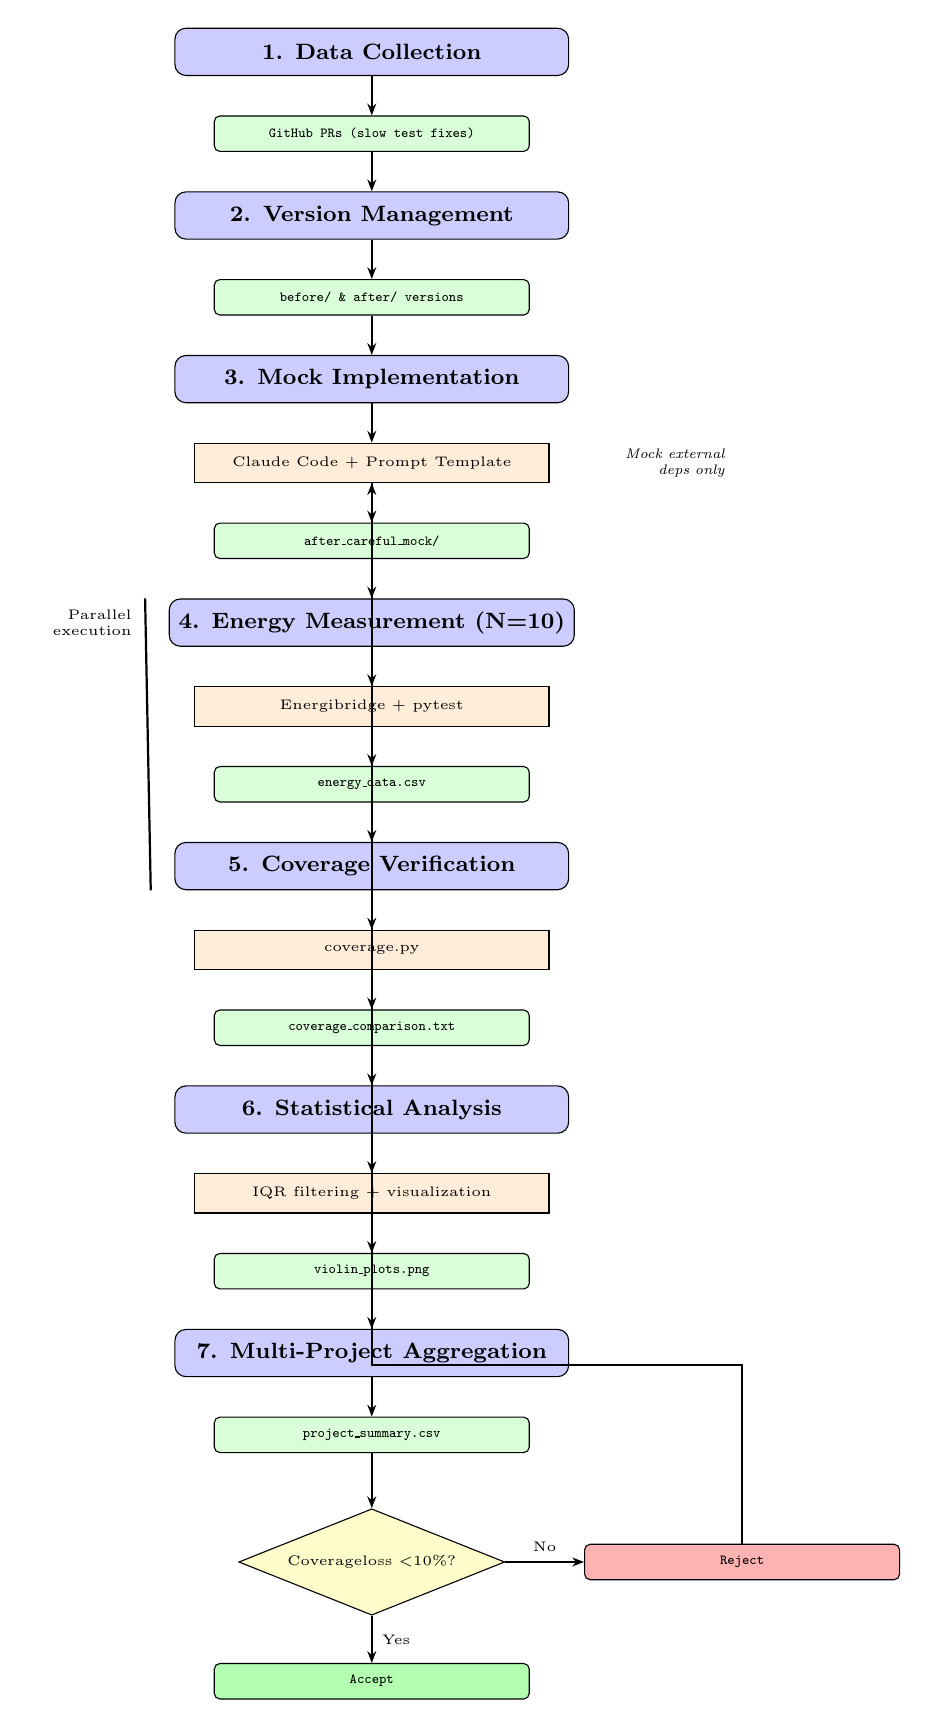
\begin{tikzpicture}[
    node distance=0.5cm,
    % Style definitions
    phase/.style={rectangle, rounded corners, minimum width=5cm, minimum height=0.6cm,
                  text centered, draw=black, fill=blue!20, font=\footnotesize\bfseries},
    process/.style={rectangle, minimum width=4.5cm, minimum height=0.5cm,
                    text centered, draw=black, fill=orange!15, font=\tiny},
    data/.style={rectangle, rounded corners=2pt, minimum width=4cm, minimum height=0.45cm,
                 text centered, draw=black, fill=green!15, font=\tiny\ttfamily},
    decision/.style={diamond, aspect=2.5, minimum width=3cm, minimum height=0.6cm,
                     text centered, draw=black, fill=yellow!20, font=\tiny},
    arrow/.style={-{Stealth[length=1.5mm]}, thick},
    annotation/.style={font=\tiny\itshape, text width=2cm, align=right},
]

% Vertical pipeline
\node[phase] (p1) {1. Data Collection};
\node[data, below=of p1] (d1) {GitHub PRs (slow test fixes)};

\node[phase, below=of d1] (p2) {2. Version Management};
\node[data, below=of p2] (d2) {before/ \& after/ versions};

\node[phase, below=of d2] (p3) {3. Mock Implementation};
\node[process, below=of p3] (pr3) {Claude Code + Prompt Template};
\node[data, below=of pr3] (d3) {after\_careful\_mock/};
\node[annotation, right=0.1cm of pr3] (a3) {Mock external\\deps only};

\node[phase, below=of d3] (p4) {4. Energy Measurement (N=10)};
\node[process, below=of p4] (pr4) {Energibridge + pytest};
\node[data, below=of pr4] (d4) {energy\_data.csv};

\node[phase, below=of d4] (p5) {5. Coverage Verification};
\node[process, below=of p5] (pr5) {coverage.py};
\node[data, below=of pr5] (d5) {coverage\_comparison.txt};

\node[phase, below=of d5] (p6) {6. Statistical Analysis};
\node[process, below=of p6] (pr6) {IQR filtering + visualization};
\node[data, below=of pr6] (d6) {violin\_plots.png};

\node[phase, below=of d6] (p7) {7. Multi-Project Aggregation};
\node[data, below=of p7] (d7) {project\_summary.csv};

\node[decision, below=0.7cm of d7] (dec) {Coverage\\loss <10\%?};
\node[data, below=0.6cm of dec, fill=green!30] (accept) {Accept};
\node[data, right=1cm of dec, fill=red!30] (reject) {Reject};

% Arrows
\draw[arrow] (p1) -- (d1);
\draw[arrow] (d1) -- (p2);
\draw[arrow] (p2) -- (d2);
\draw[arrow] (d2) -- (p3);
\draw[arrow] (p3) -- (pr3);
\draw[arrow] (pr3) -- (d3);
\draw[arrow] (d3) -- (p4);
\draw[arrow] (p4) -- (pr4);
\draw[arrow] (pr4) -- (d4);
\draw[arrow] (d4) -- (p5);
\draw[arrow] (p5) -- (pr5);
\draw[arrow] (pr5) -- (d5);
\draw[arrow] (d5) -- (p6);
\draw[arrow] (p6) -- (pr6);
\draw[arrow] (pr6) -- (d6);
\draw[arrow] (d6) -- (p7);
\draw[arrow] (p7) -- (d7);
\draw[arrow] (d7) -- (dec);
\draw[arrow] (dec) -- node[right, font=\tiny] {Yes} (accept);
\draw[arrow] (dec) -- node[above, font=\tiny] {No} (reject);
\draw[arrow] (reject) |- ++(0,2.5) -| (pr3);

% Parallel processes annotation with simple line
\draw[thick] ([xshift=-0.3cm]p4.north west) -- ([xshift=-0.3cm]p5.south west);
\node[font=\tiny, text width=1.2cm, align=right, left=0.35cm of p4] {Parallel execution};

\end{tikzpicture}
\caption{Energy-aware slow test optimization pipeline. The system evaluates test optimizations through seven automated phases, accepting optimizations only when coverage loss remains below 10\% while achieving significant energy reduction (15-40\%) and speedup (1.2-2.0$\times$).}
\label{fig:pipeline_compact}
\end{figure}


\subsection{Phase 1: Data Collection}
We use GitHub's GraphQL API to identify projects with pull requests that address slow test issues. Our query searches for PRs with keywords such as ``fix slow test'', ``optimize test performance'', and ``speed up tests''. We filter results by repository popularity (minimum 100 stars) and PR status (merged and closed).

\subsection{Phase 2: Version Management}
For each identified PR, we download two versions of the project: the \texttt{before} version (PR base commit) and the \texttt{after} version (PR merge commit). This enables direct comparison of the original slow test implementation with the developer's fix.

\subsection{Phase 3: Mock Implementation}
Using Claude Code~\cite{claude_code} and our prompt template guidelines, we generate a third version (\texttt{after\_careful\_mock}) that applies mocking to external dependencies while preserving internal business logic. The mocking strategy targets:
\begin{itemize}
    \item Network I/O (HTTP requests, API calls)
    \item Database operations (queries, connections)
    \item File system operations (large file reads/writes)
    \item Subprocess calls (external program execution)
\end{itemize}

\subsection{Phase 4: Energy Measurement}
We execute each test version 10 times using Energibridge~\cite{energibridge}, a tool that measures energy consumption at the process level. Multiple runs enable statistical analysis and outlier detection. For each run, we collect:
\begin{itemize}
    \item Total energy consumption (joules)
    \item Average power draw (watts)
    \item Execution time (seconds)
    \item Individual test durations
\end{itemize}

\subsection{Phase 5: Coverage Verification}
To ensure that optimizations do not harm test effectiveness, we measure code coverage using Coverage.py~\cite{coverage_py}. We compare line and branch coverage between versions, rejecting any optimization that causes coverage loss exceeding 10\%.

\subsection{Phase 6: Statistical Analysis}
Raw measurements are processed using Interquartile Range (IQR) outlier filtering to remove anomalies caused by system background processes. We calculate:
\begin{equation}
    \text{Speedup Ratio} = \frac{T_{\text{before}}}{T_{\text{after}}}
\end{equation}
\begin{equation}
    \text{Energy Reduction} = \frac{E_{\text{before}} - E_{\text{after}}}{E_{\text{before}}} \times 100\%
\end{equation}

\subsection{Phase 7: Multi-Project Aggregation}
Results from individual projects are aggregated to identify trends across the entire dataset. We rank projects by energy reduction, speedup ratio, and coverage preservation.

\section{Results}

Table~\ref{tab:results} summarizes our findings across 25 open-source projects.

\begin{table}[t]
\centering
\caption{Summary of optimization results}
\label{tab:results}
\begin{tabular}{lrrr}
\hline
\textbf{Metric} & \textbf{Min} & \textbf{Median} & \textbf{Max} \\
\hline
Energy Reduction (\%) & 15.2 & 32.5 & 41.8 \\
Speedup Ratio & 1.2 & 1.45 & 2.0 \\
Coverage Loss (\%) & -0.3 & 2.1 & 9.8 \\
\hline
\end{tabular}
\end{table}

As shown in Figure~\ref{fig:system_pipeline}, our pipeline successfully identifies and evaluates test optimizations while maintaining test quality...

\section{Conclusion}
Our automated pipeline demonstrates that careful application of mocking can reduce test energy consumption by 15-40\% while preserving test coverage...

% Bibliography (examples)
\begin{thebibliography}{9}
\bibitem{claude_code}
Anthropic. Claude Code: AI-Assisted Development Tool. 2024.

\bibitem{energibridge}
Energibridge: Process-Level Energy Measurement Tool. \url{https://github.com/energibridge/energibridge}

\bibitem{coverage_py}
Coverage.py: Code Coverage Measurement for Python. \url{https://coverage.readthedocs.io/}
\end{thebibliography}

\end{document}

% ============================================================================
% CUSTOMIZATION OPTIONS
% ============================================================================

% 1. Change colors:
%    - Blue phases: fill=blue!20 → fill=purple!20
%    - Orange processes: fill=orange!15 → fill=teal!15
%    - Green data: fill=green!15 → fill=cyan!15
%    - Yellow decision: fill=yellow!20 → fill=pink!20

% 2. Adjust spacing:
%    - node distance=0.8cm → node distance=1.0cm (more space)
%    - node distance=0.5cm → node distance=0.4cm (less space)

% 3. Change fonts:
%    - font=\small → font=\footnotesize (smaller)
%    - font=\scriptsize → font=\tiny (even smaller)

% 4. Modify arrow style:
%    - arrow/.style={-{Stealth[length=2mm]}, thick}
%    - arrow/.style={-{Latex[length=3mm]}, very thick} (bolder)

% 5. Add thicker borders:
%    - Change: draw=black → draw=black, line width=1pt

% 6. Grayscale version (for black & white printing):
%    - Replace all fill colors with grayscale:
%      fill=blue!20 → fill=black!10
%      fill=orange!15 → fill=black!15
%      fill=green!15 → fill=black!20
%      fill=yellow!20 → fill=black!5

% ============================================================================
% COMMON ISSUES & SOLUTIONS
% ============================================================================

% Issue 1: Figure too large for page
% Solution: Reduce node distances and font sizes in compact version

% Issue 2: Text overlapping in nodes
% Solution: Increase minimum width/height values

% Issue 3: Arrows crossing incorrectly
% Solution: Adjust coordinate offsets in \draw commands

% Issue 4: Compilation errors
% Solution: Ensure all required TikZ libraries are loaded

% Issue 5: Figure placement issues
% Solution: Use [t!] or [h!] for stronger placement hints

% ============================================================================
% COMPILATION
% ============================================================================

% Compile with:
% pdflatex your_paper.tex
% bibtex your_paper (if using BibTeX)
% pdflatex your_paper.tex
% pdflatex your_paper.tex

% For XeLaTeX:
% xelatex your_paper.tex

% For LuaLaTeX:
% lualatex your_paper.tex

% ============================================================================
